%%%%%%%%%%%%%%%%%%%%%%%%%%%%%%%%%%%%%%%%%
% Jacobs Landscape Poster
% LaTeX Template
% Version 1.1 (14/06/14)
%
% Created by:
% Computational Physics and Biophysics Group, Jacobs University
% https://teamwork.jacobs-university.de:8443/confluence/display/CoPandBiG/LaTeX+Poster
% 
% Further modified by:
% Nathaniel Johnston (nathaniel@njohnston.ca)
%
% This template has been downloaded from:
% http://www.LaTeXTemplates.com
%
% License:
% CC BY-NC-SA 3.0 (http://creativecommons.org/licenses/by-nc-sa/3.0/)
%
%%%%%%%%%%%%%%%%%%%%%%%%%%%%%%%%%%%%%%%%%

%----------------------------------------------------------------------------------------
%	PACKAGES AND OTHER DOCUMENT CONFIGURATIONS
%----------------------------------------------------------------------------------------

\documentclass[final]{beamer}

\usepackage[scale=1.24]{beamerposter} % Use the beamerposter package for laying out the poster

\usetheme{confposter} % Use the confposter theme supplied with this template

\setbeamercolor{block title}{fg=dblue,bg=white} % Colors of the block titles
\setbeamercolor{block body}{fg=black,bg=white} % Colors of the body of blocks
\setbeamercolor{block alerted title}{fg=white,bg=dblue!70} % Colors of the highlighted block titles
\setbeamercolor{block alerted body}{fg=black,bg=dblue!10} % Colors of the body of highlighted blocks
% Many more colors are available for use in beamerthemeconfposter.sty

%-----------------------------------------------------------
% Define the column widths and overall poster size
% To set effective sepwid, onecolwid and twocolwid values, first choose how many columns you want and how much separation you want between columns
% In this template, the separation width chosen is 0.024 of the paper width and a 4-column layout
% onecolwid should therefore be (1-(# of columns+1)*sepwid)/# of columns e.g. (1-(4+1)*0.024)/4 = 0.22
% Set twocolwid to be (2*onecolwid)+sepwid = 0.464
% Set threecolwid to be (3*onecolwid)+2*sepwid = 0.708

\newlength{\sepwid}
\newlength{\onecolwid}
\newlength{\twocolwid}
\newlength{\threecolwid}
\setlength{\paperwidth}{48in} % A0 width: 46.8in
\setlength{\paperheight}{36in} % A0 height: 33.1in
\setlength{\sepwid}{0.024\paperwidth} % Separation width (white space) between columns
\setlength{\onecolwid}{0.22\paperwidth} % Width of one column
\setlength{\twocolwid}{0.464\paperwidth} % Width of two columns
\setlength{\threecolwid}{0.708\paperwidth} % Width of three columns
\setlength{\topmargin}{-0.5in} % Reduce the top margin size
%-----------------------------------------------------------

\usepackage{graphicx}

\usepackage{booktabs} % Top and bottom rules for tables
\usepackage{eso-pic}
\usepackage{pgfpages}
\pgfpagesuselayout{resize to}[a4paper,landscape,border shrink=5mm]




%----------------------------------------------------------------------------------------
%	TITLE SECTION 
%----------------------------------------------------------------------------------------
\title{Legal \& Ethical Issues of Cloud Storage} % Poster title

\author{M.Cromie, F.Leishman, E.Malinovskis, A.McDonald \& M.Paterson} % Author(s)

\institute{School of Computing Science, University of Glasgow} % Institution(s)

%----------------------------------------------------------------------------------------




\begin{document}
\addtobeamertemplate{block end}{}{\vspace*{2ex}} % White space under blocks
\addtobeamertemplate{block alerted end}{}{\vspace*{2ex}} % White space under highlighted (alert) blocks

\setlength{\belowcaptionskip}{2ex} % White space under figures
\setlength\belowdisplayshortskip{2ex} % White space under equations

\begin{frame}[t] % The whole poster is enclosed in one beamer frame

\begin{columns}[t] % The whole poster consists of three major columns, the second of which is split into two columns twice - the [t] option aligns each column's content to the top

\begin{column}{\sepwid}\end{column} % Empty spacer column

\begin{column}{\onecolwid} % The first column

%----------------------------------------------------------------------------------------
%	INTRODUCTION
%----------------------------------------------------------------------------------------

\begin{alertblock}{Introduction}
As individuals and businesses alike are becoming increasingly aware of the benefits of cloud storage, the importance of issues surrounding the privacy and security of their data raises several legal and ethical issues which this poster will aim to explore.
\end{alertblock}

\begin{figure}
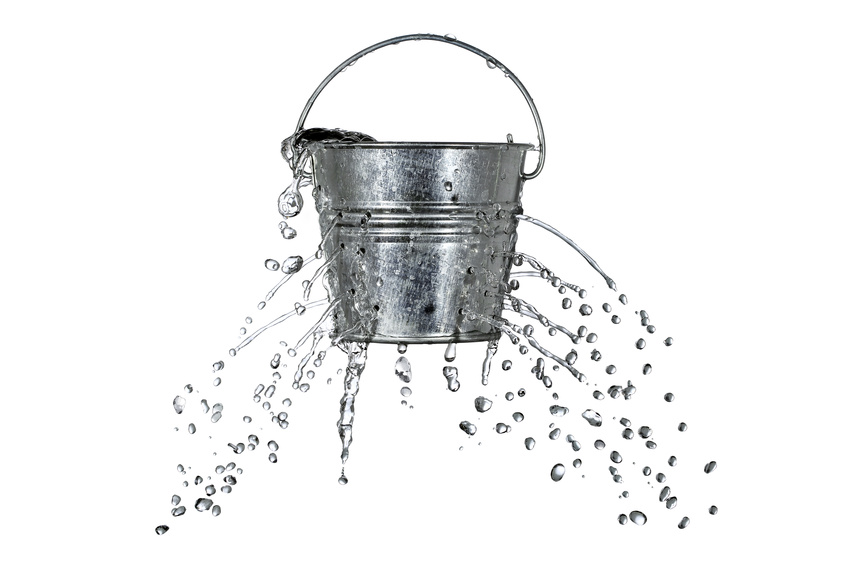
\includegraphics[width=0.8\linewidth]{leak.jpg}
% \caption{...}
\end{figure}




\begin{block}{Leaks}
\begin{itemize}
\item Cloud storage leaks are becoming increasingly common.
\item But who's fault is it when data is stolen? The user or the storage company?
\item A recent example would be the iCloud photo hack resulting in private pictures of celebrities being stolen. This was made possible by a combination of weak passwords and security vulnerabilities of iCloud being exploited. 
\item Ethical issues could be raised when users believed that their iCloud accounts were secure, despite security vulnarablities of iCloud this data was leaked. 
\item Another ethical issue with this is that some users were unaware that their data was uploaded on the cloud\cite{iCloud}, with automatic backups enabled without their explicit permission.
\end{itemize}

\end{block}

%------------------------------------------------



%----------------------------------------------------------------------------------------

\end{column} % End of the first column

\begin{column}{\sepwid}\end{column} % Empty spacer column

\begin{column}{\twocolwid} % Begin a column which is two columns wide (column 2)

\begin{columns}[t,totalwidth=\twocolwid] % Split up the two columns wide column

\begin{column}{\onecolwid}\vspace{-.6in} % The first column within column 2 (column 2.1)

%----------------------------------------------------------------------------------------
%	MATERIALS
%----------------------------------------------------------------------------------------

\begin{block}{Sharing Data}
\begin{itemize}
\item What is to stop employees from accessing, reading, sharing or selling user data?
\item This is a very difficult issue, with a fine line between what is acceptable to be used by the storage company.
\item An example of this is one of Dropbox's terms that they have full access to all data uploaded to their service, allowing them full ownership\cite{onwubiko}.
\item This raises severe ethical concerns, with users questioning the reasons behind this policy.
\item The new revision of the General Data Protection Regulation aims to help the protection of private data, in order to stop this happening. 
\item This will be aimed at targetting cloud storage companies, as the law will enforce strict controls on personal data; harsher security requirements and even harsher penalties for companies that breach these laws. 
\end{itemize}
\end{block}

\begin{figure}

\includegraphics[width=0.8\linewidth]{storage.jpeg}
\caption{A simple diagram illustrating the basic concepts of cloud storage}
\end{figure}

%----------------------------------------------------------------------------------------

\end{column} % End of column 2.1

\begin{column}{\onecolwid}\vspace{-.6in} % The second column within column 2 (column 2.2)

%----------------------------------------------------------------------------------------
%	METHODS
%----------------------------------------------------------------------------------------
\begin{block}{Backup}
\begin{itemize}
\item Backups are made regularly by the storage company to prevent loss of user data.
\item These back ups are usually stored off site, to keep data safe. 
\item Users have little or no control over access to the backup data (both remote and physical).
\item Backup service provided is often ``Best effort'' and the providers do not take over any liability associated with data loss or misplacement.
\item This raises potential ethical issues, with the user trusting the storage company to make regular incremental back ups and the company failing to do so.
\item This is often signed into a contract, which users should research before selecting a provider.
\end{itemize}
\end{block}

\begin{block}{Encryption}
\begin{itemize}
\item Data stored on the cloud is not as secure as many people believe.
\item As a solution encryption shouldbe utilised to further protect the information.
\item However, encryption is not without its flaws. Who encrypts the data? Who has access to the keys?
\item Some storage companies provide services for users to encrpyt the data but the companies will retain access of the keys\cite{good}.
\item This is a critical issue for businesses storing customer data on the cloud, as they could be violating the Data Protection Act should they be enabling unauthorised people to view potentially sensitive information.
\end{itemize}
\end{block}


%----------------------------------------------------------------------------------------

\end{column} % End of column 2.2

\end{columns} % End of the split of column 2 - any content after this will now take up 2 columns width

%----------------------------------------------------------------------------------------
%	IMPORTANT RESULT
%----------------------------------------------------------------------------------------


%----------------------------------------------------------------------------------------

\begin{columns}[t,totalwidth=\twocolwid] % Split up the two columns wide column again

\begin{column}{\onecolwid} % The first column within column 2 (column 2.1)

%----------------------------------------------------------------------------------------
%	MATHEMATICAL SECTION
%----------------------------------------------------------------------------------------


%----------------------------------------------------------------------------------------

\end{column} % End of column 2.1

\begin{column}{\onecolwid} % The second column within column 2 (column 2.2)

%----------------------------------------------------------------------------------------
%	RESULTS
%----------------------------------------------------------------------------------------
%----------------------------------------------------------------------------------------

\end{column} % End of column 2.2

\end{columns} % End of the split of column 2

\end{column} % End of the second column

\begin{column}{\sepwid}\end{column} % Empty spacer column

\begin{column}{\onecolwid} % The third column

%----------------------------------------------------------------------------------------
%	CONCLUSION
%----------------------------------------------------------------------------------------
\begin{figure}
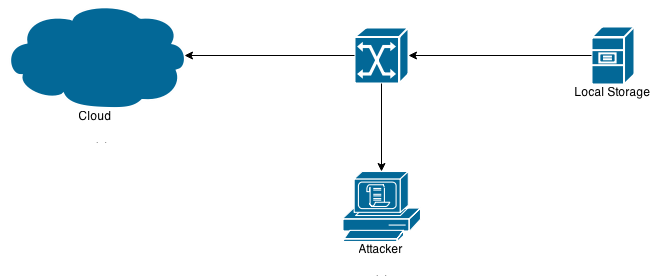
\includegraphics[width=0.8\linewidth]{Maninthemiddle.png}
\caption{A diagram illustrating what can happen without encryption}
\end{figure}
\begin{alertblock}{Conclusion}
While we believe there are many pros and cons for businesses and individuals to consider before electing to store their data on the cloud, we feel that the pros vastly outweigh the cons as the ability to access information from anywhere in the world is too beneficial for many to ignore. \\
\vspace{2mm} However, cloud storage providers should be more transparent with their terms and conditions with reference to the way in which they are using the data that they are being paid to store and secure. 
\end{alertblock}



%----------------------------------------------------------------------------------------
%	REFERENCES
%----------------------------------------------------------------------------------------

\begin{block}{References}

\nocite{*} % Insert publications even if they are not cited in the poster
\small{\bibliographystyle{unsrt}
\bibliography{example}\vspace{0.75in}}

\end{block}


%----------------------------------------------------------------------------------------

\end{column} % End of the third column

\end{columns} % End of all the columns in the poster

\end{frame} % End of the enclosing frame

\end{document}
